\section{Result}
\label{sec:result}

\subsection{Homogeneous grid}
A homogeneous grid containing $1024$ nodes where each node has been perturbed a small amount was used to execute the algorithm with several different choices of parameters, with a focus on the maintenance parameter, $\mu$. This is shown in Figure \ref{fig:homogeneous}, which shows that when $\mu = 1$, i.e. the linear case, the solution that is found is the shortest path between each source and sink. When $\mu > 1$, the path chosen may not be the shortest path and there also exists a preference to share paths.

\begin{figure}
\centering
\begin{subfigure}[b]{0.48\textwidth}
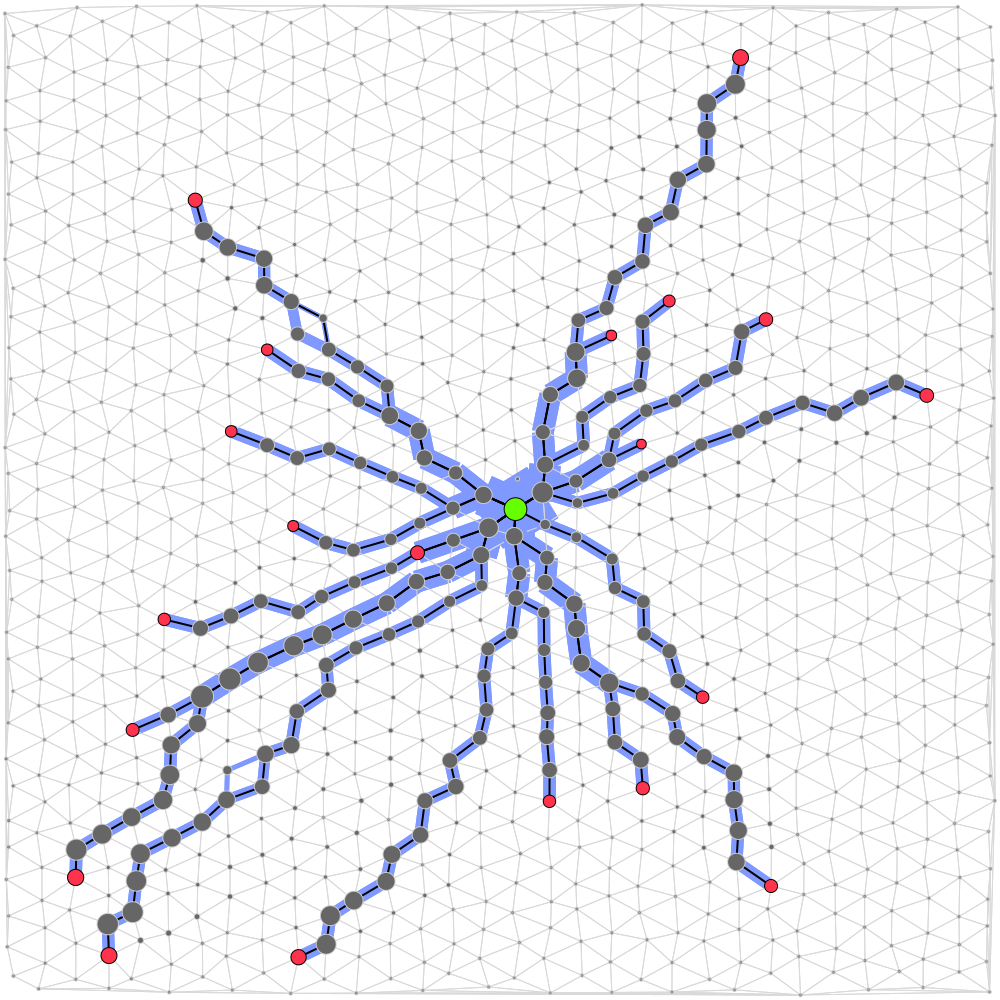
\includegraphics[width=\textwidth]{{img/nodes_sources_M10_mu1.0}.png}
\caption{The simulated solution when $\mu=1$. Converged at approximately $xxxx$ time steps.}
\end{subfigure}
~
\begin{subfigure}[b]{0.48\textwidth}
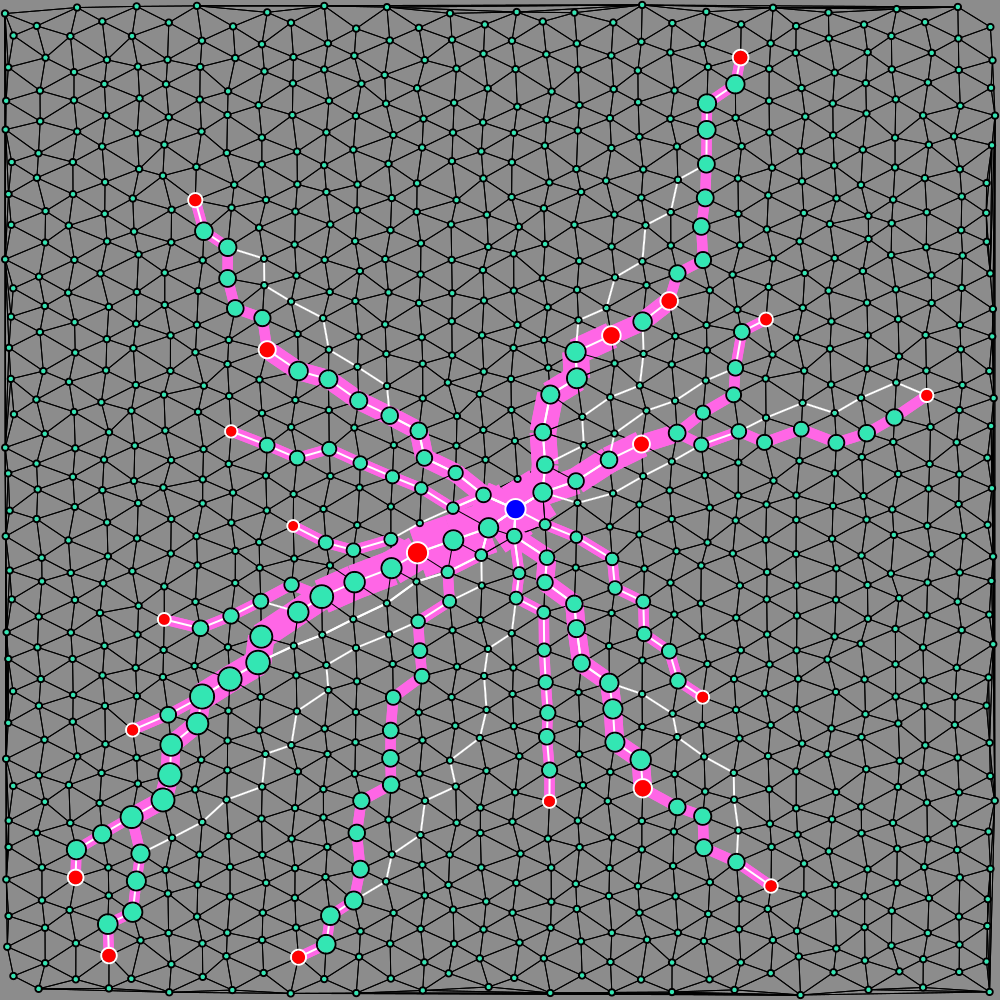
\includegraphics[width=\textwidth]{{img/nodes_sources_M10_mu1.05}.png}
\caption{The simulated solution when $\mu=1.05$.  Converged at approximately $20000$ time steps.}
\end{subfigure}

\begin{subfigure}[b]{0.48\textwidth}
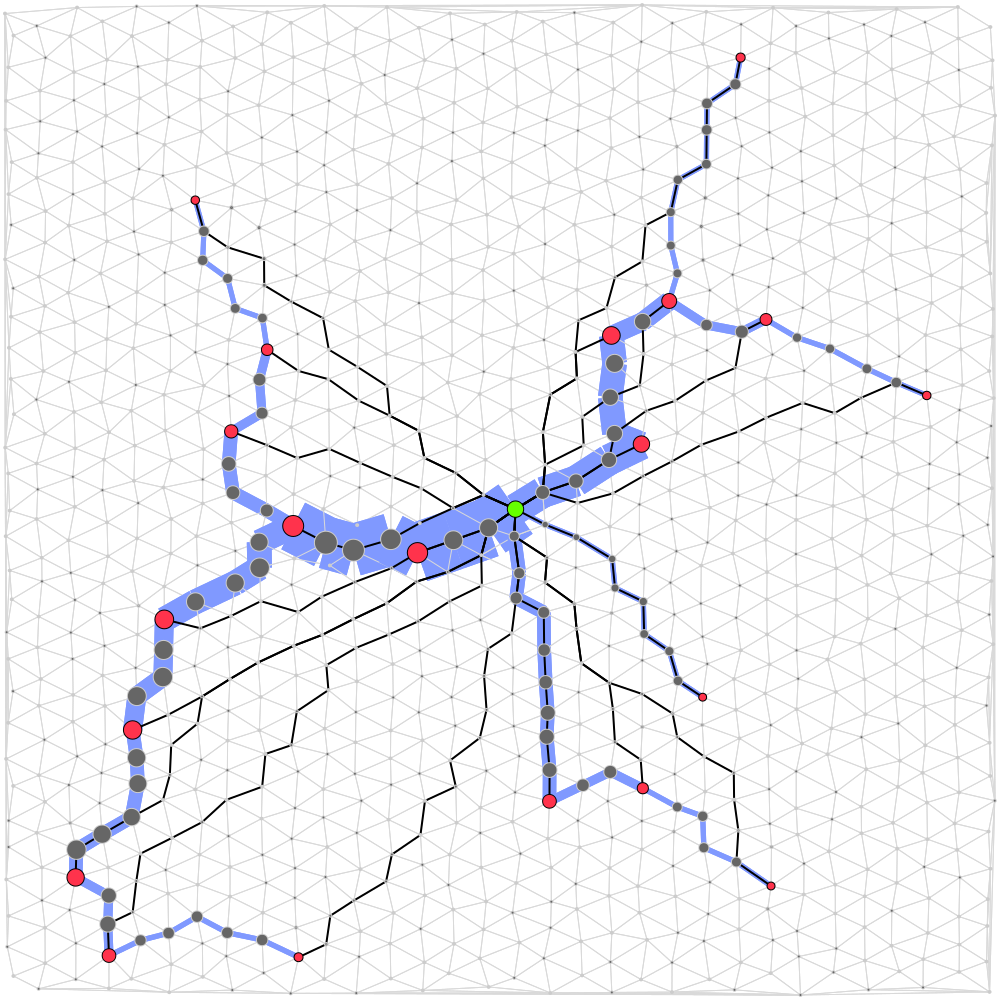
\includegraphics[width=\textwidth]{{img/nodes_sources_M10_mu1.4}.png}
\caption{The simulated solution when $\mu=1.4$.  Converged at approximately $45000$ time steps.}
\end{subfigure}
~
\begin{subfigure}[b]{0.48\textwidth}
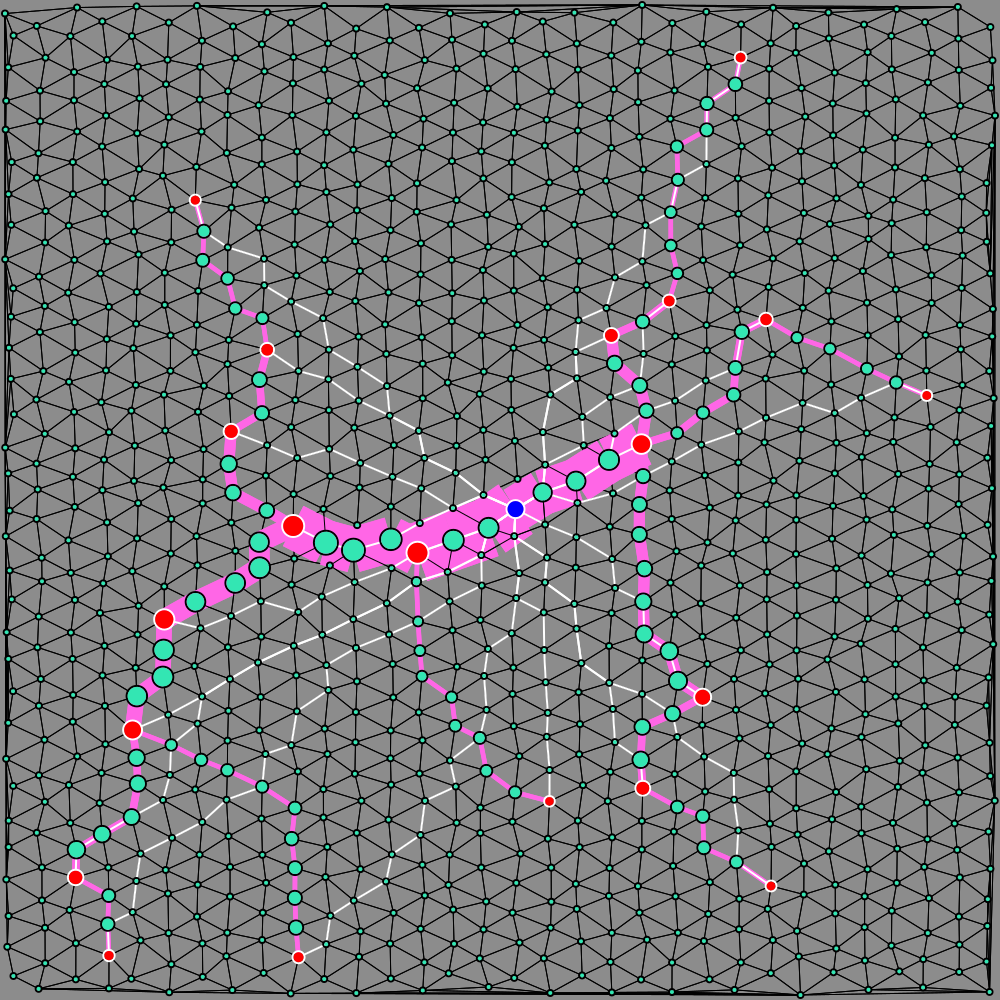
\includegraphics[width=\textwidth]{{img/nodes_sources_M10_mu1.5}.png}
\caption{The simulated solution when $\mu=1.5$.  Converged at approximately $50000$ time steps.}
\end{subfigure}
\caption{Figure shows the converged solutions found by the simulation on a homogeneous grid containing $1024$ nodes where each node has been perturbed a small amount. The pink lines show the conductivity along each edge, with the thickness of the line is proportional to the amount of conductivity. The shortest path found with Dijkstra's algorithm from each source to each sinks has been marked with a thin white line \cite{Dijkstra}. The parameters used are $q = 10^{-4},\lambda = 10^{-3},$ and $D_{min}=5 \cdot 10^{-2}$. In this graph there are in total one sink and $20$ sources. Each source (red) produces 1000 particles each time unit and all sinks (blue) can together remove as many particles as are produced each time unit (evenly divided between the sinks).}
\label{fig:sources}
\end{figure}

\begin{figure}
\centering
\begin{subfigure}[b]{0.48\textwidth}
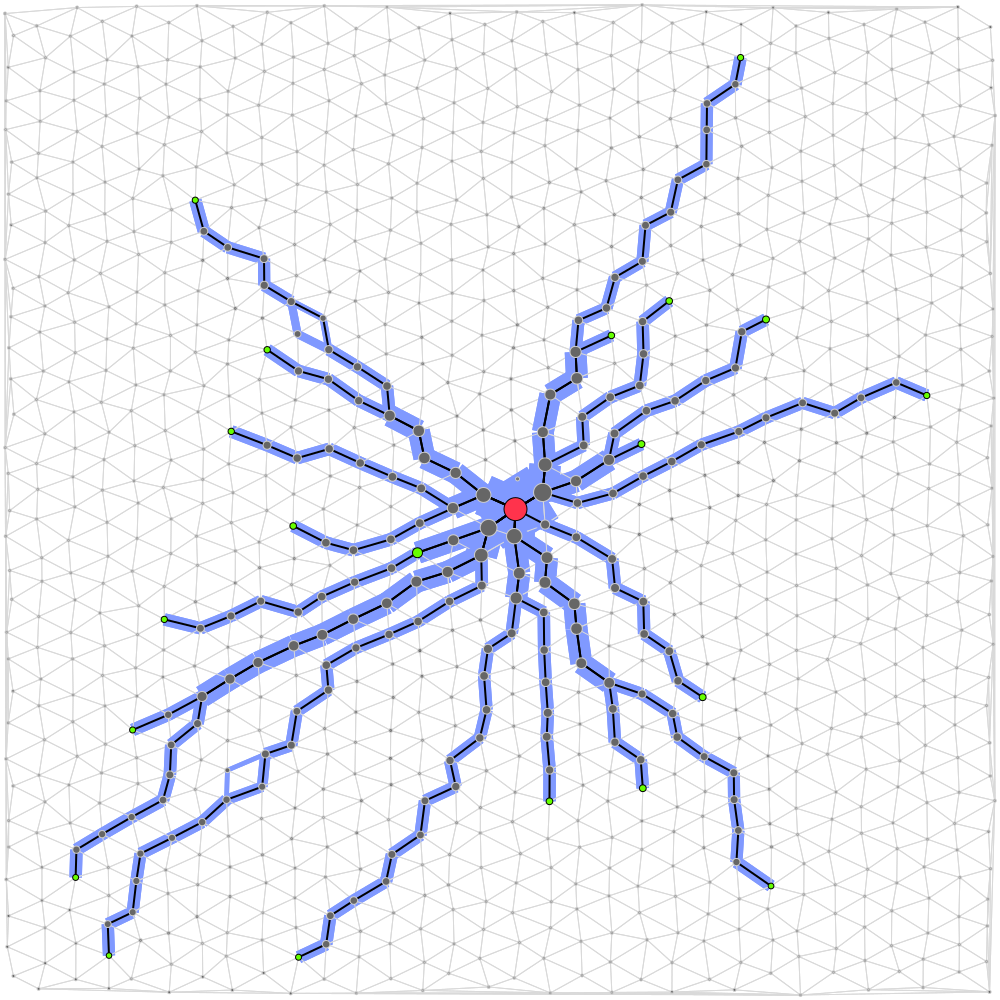
\includegraphics[width=\textwidth]{{img/nodes_sinks_M10_mu1.0}.png}
\caption{The simulated solution when $\mu=1$. Converged at approximately $xxxx$ time steps.}
\end{subfigure}
~
\begin{subfigure}[b]{0.48\textwidth}
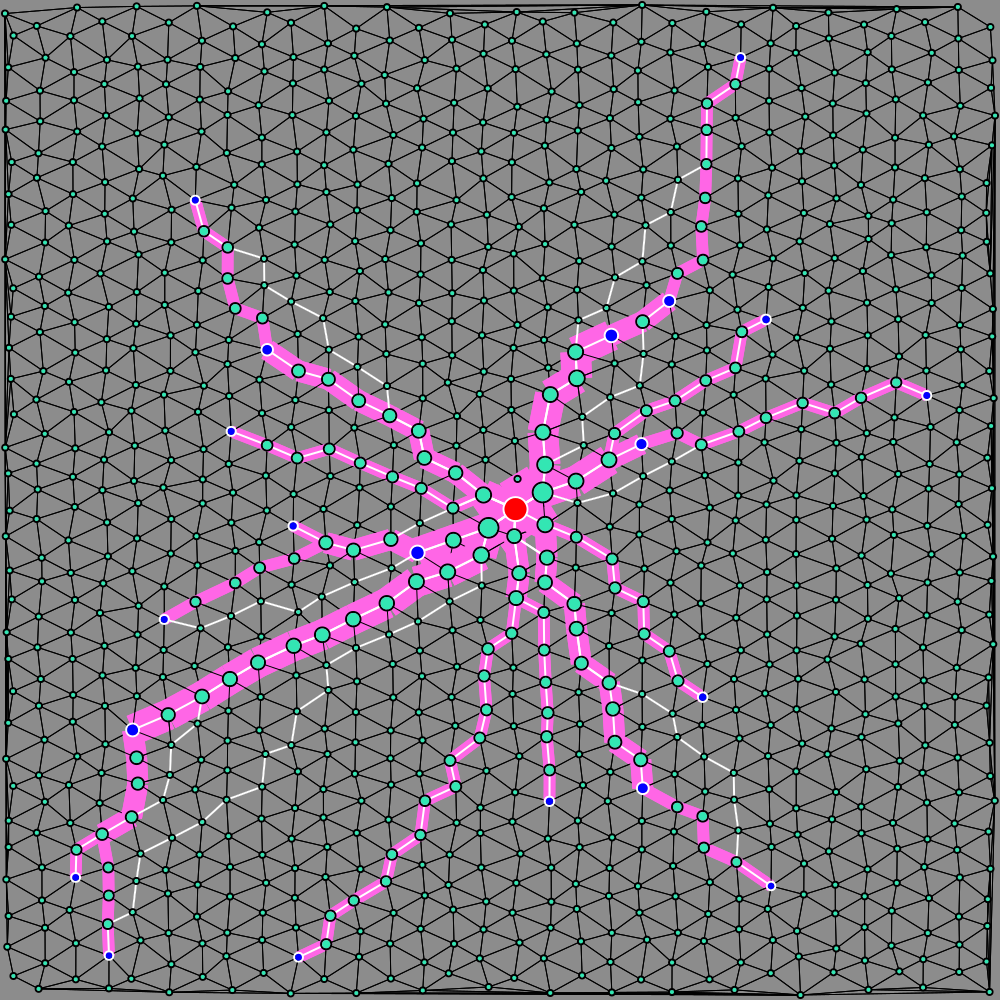
\includegraphics[width=\textwidth]{{img/nodes_sinks_M10_mu1.05}.png}
\caption{The simulated solution when $\mu=1.05$. Converged at approximately $120000$ time steps.}
\end{subfigure}

\begin{subfigure}[b]{0.48\textwidth}
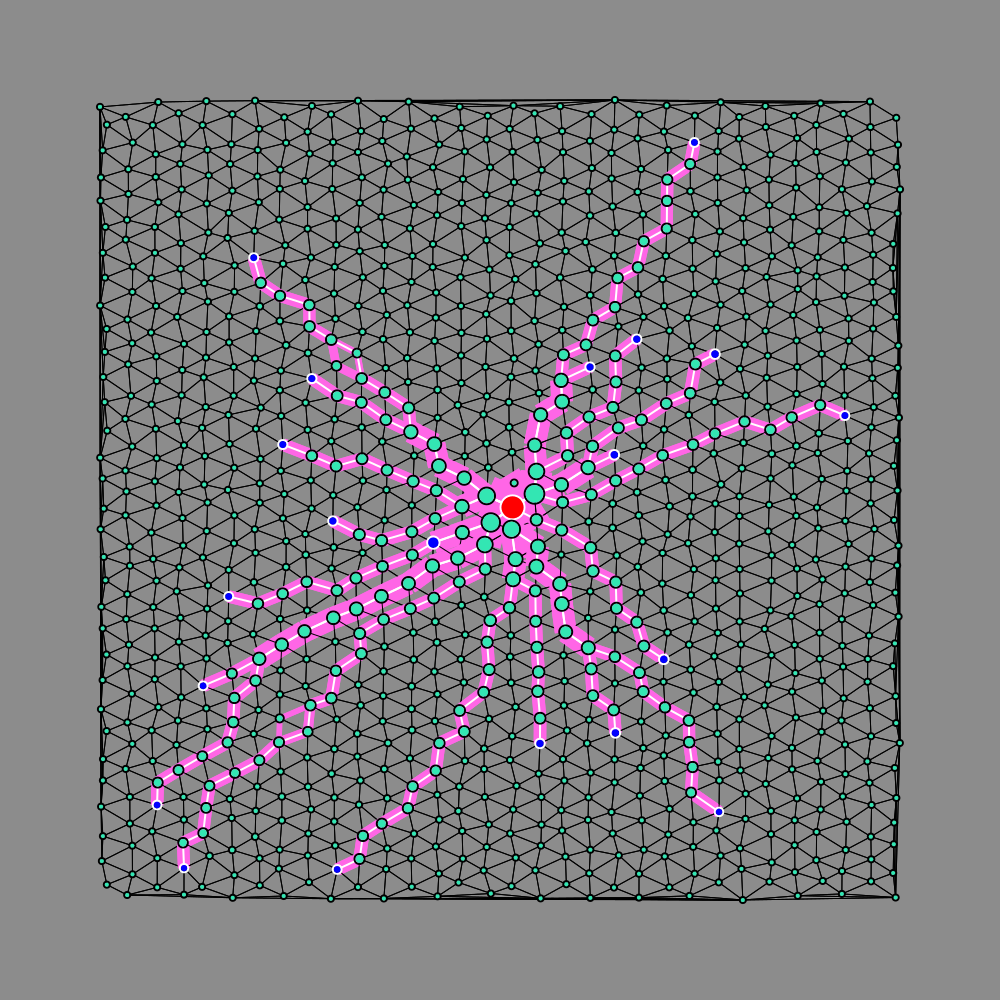
\includegraphics[width=\textwidth]{{img/nodes_sinks_M10_mu1.4}.png}
\caption{The simulated solution when $\mu=1.4$. Converged at approximately $xxxx$ time steps.}
\end{subfigure}
~
\begin{subfigure}[b]{0.48\textwidth}
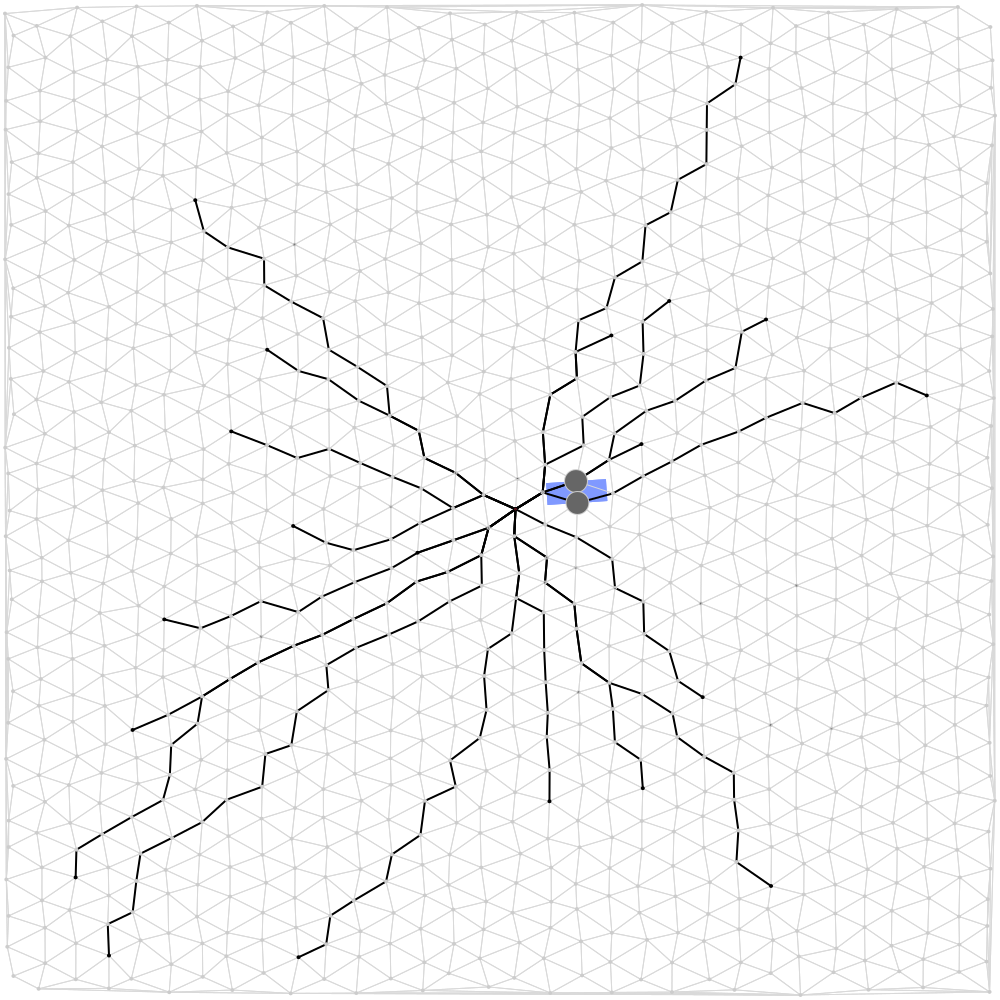
\includegraphics[width=\textwidth]{{img/nodes_sinks_M10_mu1.5}.png}
\caption{The simulated solution when $\mu=1.5$. Converged at approximately $xxxx$ time steps.}
\end{subfigure}
\caption{Figure shows the solutions found by the simulation on a homogeneous grid containing $1024$ nodes where each node has been perturbed a small amount. The pink lines show the conductivity along each edge, with the thickness of the line is proportional to the amount of conductivity. The shortest path found with Dijkstra's algorithm from each source to each sinks has been marked with a thin white line \cite{Dijkstra}. The parameters used are $q = 10^{-4},\lambda = 10^{-3},$ and $D_{min}=5 \cdot 10^{-2}$. In this graph there are in total one source and $20$ sinks. Each source (red) produces 1000 particles each time unit and all sinks (blue) can together remove as many particles as are produced each time unit (evenly divided between the sinks).}
\label{fig:sinks}
\end{figure}

\subsection{City}

Another grid was created using road data from the city of Uppsala, Sweden.

\subsection{Parallelism}
The measures used to benchmark the performance of the parallel OpenMP implementation was speedup and sizeup. Figure \ref{fig:speed_size} shows the result from the speedup and sizeup measurements. All benchmarking were done on the Uppsala University servers \textit{vitsippa.it.uu.se} and \textit{tussilago.it.uu.se}, both with specifications: 

\begin{itemize}
\item CPU: AMD Opteron (Bulldozer) 6282SE, 2.6 GHz, 16-core, dual socket
\item Memory: 128 GB
\item OS: Scientific Linux 6.5.
\end{itemize}

\noindent All \texttt{C++} code was compiled with \texttt{gcc 4.8.2} with the \texttt{-fopenmp}, \texttt{-O3} and  \texttt{-static-libstdc++} flags.

\begin{figure}
\centering
\begin{subfigure}[b]{1\textwidth}
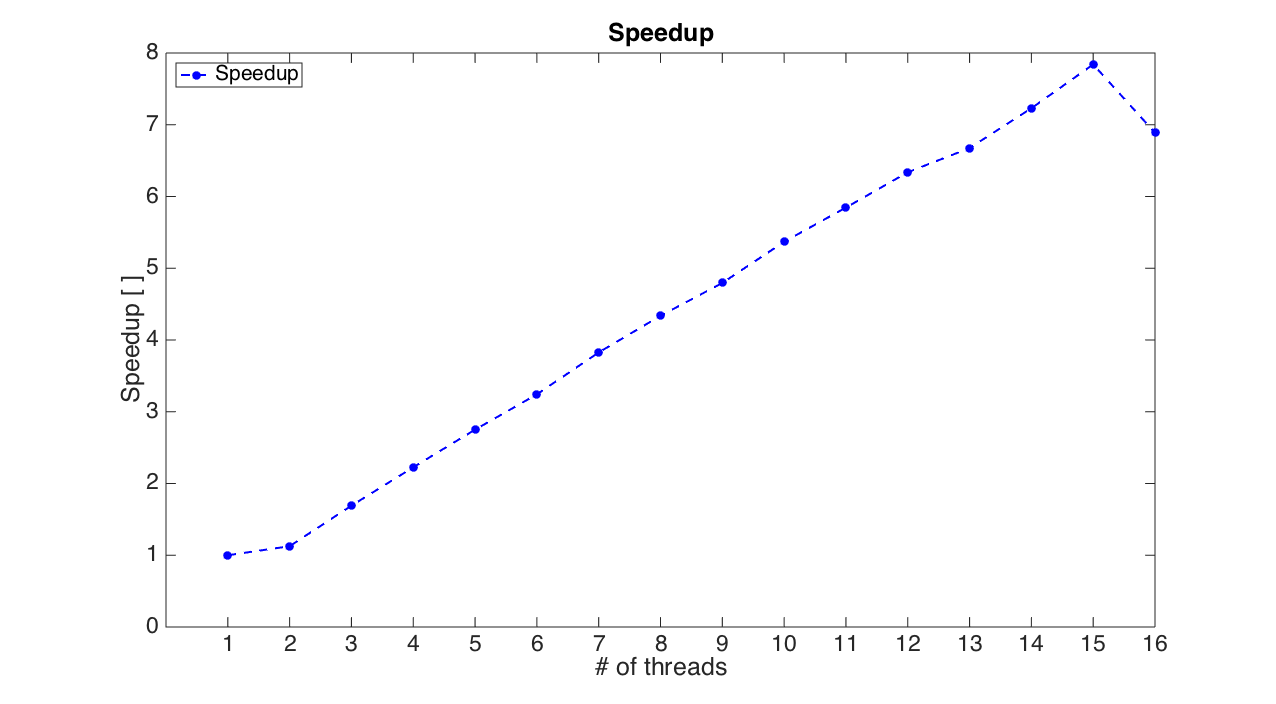
\includegraphics[width=\textwidth, height=0.5\textwidth]{img/speedup.png}
\caption{The speedup of the parallel implementation. A uniformly randomized grid containing $10000$ nodes was used for measuring the speedup. The simulation was run for $1000$ iterations with a time step of $0.1$.}
\end{subfigure}

\begin{subfigure}[b]{1\textwidth}
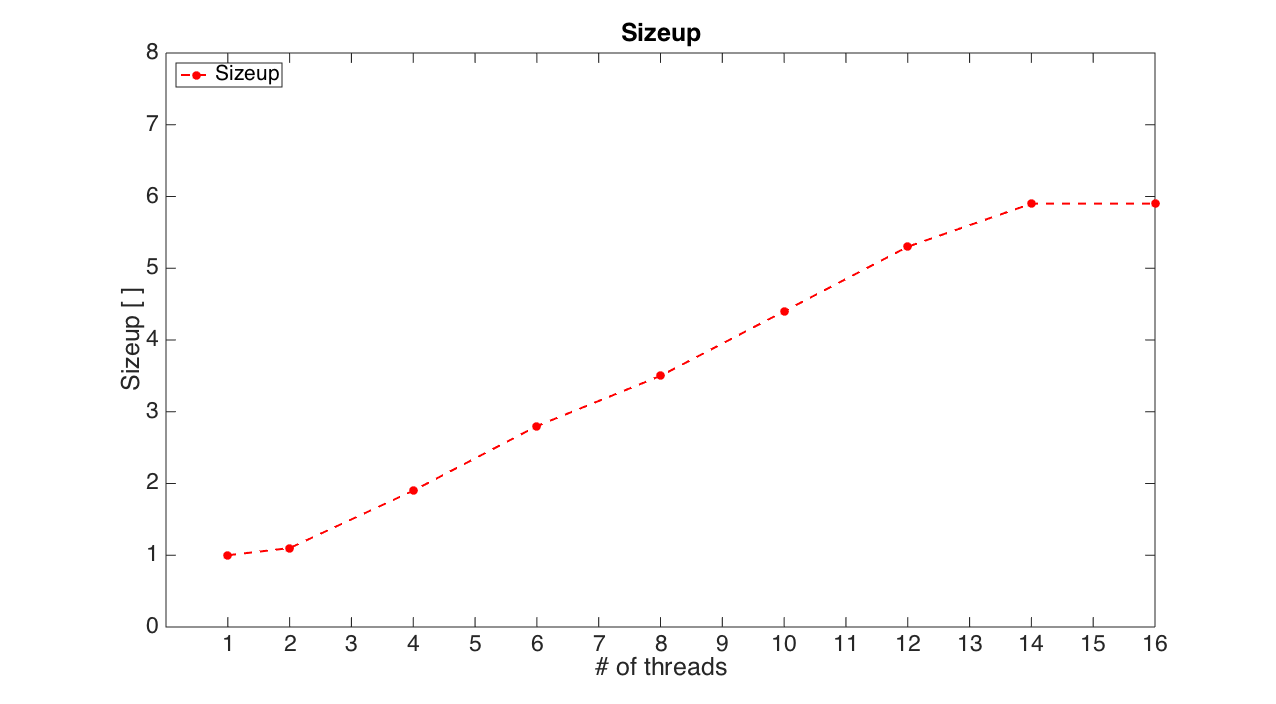
\includegraphics[width=\textwidth, height=0.5\textwidth]{img/sizeup.png}
\caption{The sizeup of the parallel implementation. The reference size, i.e. the size of the problem when sizeup is one was a uniformly randomized grid containing $5000$ nodes. The computation time used for measuring the sizeup was $60~s$ with an allowed variation of $\pm 3~s$. }
\end{subfigure}
\caption{Figure shows the different measurements of the parallel implementation of the algorithm presented in Algorithm \ref{alg:outline}. All benchmarking was run three times per data point and the best performance among those data points was extracted and used in these results.}
\label{fig:speed_size}
\end{figure}

